%%%%%%%%%%%%%%%%%%%%% {{{
%%Options for presentations (in-class) and handouts (e.g. print).
% \documentclass[pdf,9pt]{beamer}
\documentclass[pdf,9pt]{beamer}


%%%%%%%%%%%%%%%%%%%%%%
%Change this for different slides so it appears in bar
\usepackage{authoraftertitle}
\date{Chapter 4. Vector Geometry\\ \S 4-1. Vectors and Lines}

%%%%%%%%%%%%%%%%%%%%%%
%% Upload common style file
\usepackage{LyryxLAWASlidesStyle}

\begin{document}

%%%%%%%%%%%%%%%%%%%%%%%
%% Title Page and Copyright Common to All Slides

%Title Page
\input frontmatter/titlepage_to_Jim.tex

%LOTS Page
\input frontmatter/lyryxopentexts.tex

%Copyright Page
\input frontmatter/copyright.tex

%%%%%%%%%%%%%%%%%%%%%%%%% }}}
%-------------- start slide -------------------------------%{{{ 2
\begin{frame}[fragile]
   \tableofcontents
\end{frame}
%-------------- end slide -------------------------------%}}}
%-------------- start slide -------------------------------%{{{ 3
\begin{frame}
 \begin{center}
   {\bf NOTE:} Much of this chapter is what you would learn in Multivariable Calculus. \\ You might find it interesting/useful to read. \\ But I will only cover the material important to this course.
     \end{center}
\end{frame}
%-------------- end slide -------------------------------%}}}
\section[\textcolor{yellow}{}]{\textcolor{yellow}{Vector Norms (i.e., lengths)}}
%-------------- start slide -------------------------------%{{{ 4
\begin{frame}
    \frametitle{Vector Norms}
    \pause
    \begin{itemize}
	\item
	    The word ``norm" in linear algebra is used to mean ``length".
	\item
	    There are actually many ways to define length, the most usual Euclidean:
	    \begin{itemize}
		\item
		    In 2D and 3D: \\[3pt]
		    % 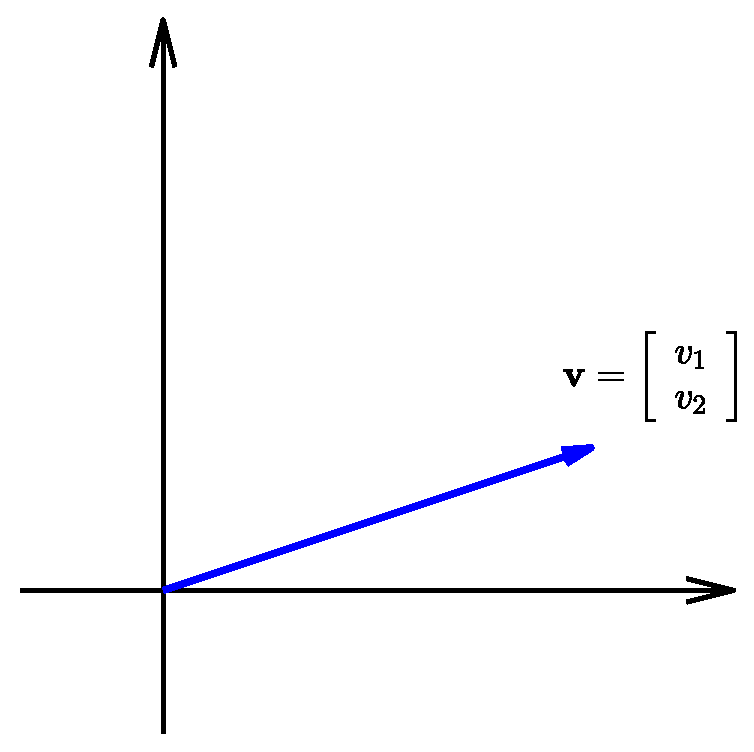
\includegraphics[width=3.5cm]{figures/LengthPlot2D}
	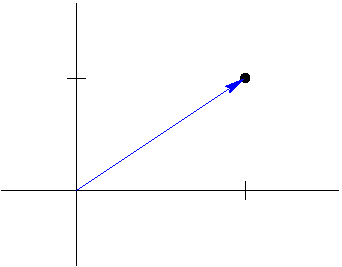
\includegraphics[scale=0.09]{R2.png}
	\hfill
	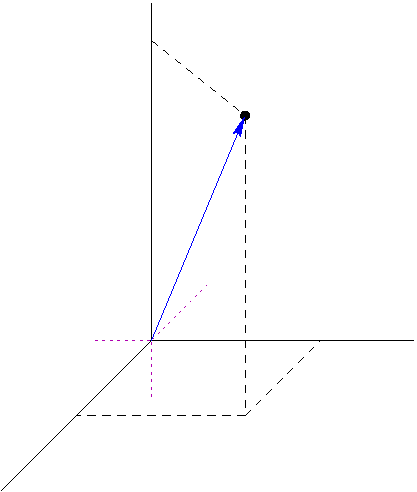
\includegraphics[scale=0.09]{R3.png}
		\item[]
		\item
		    In general, if $\vec{v} \in \RR^n$, the Euclidean \alert{norm} of $\vec{v}$ is:
		    $$
		    \|\vec{v}\| = \sqrt{\vec{v} \cdot \vec{v}} = \sqrt{\vec{v}^T\vec{v}} = \sqrt{v_1^2 + v_2^2 + \cdots + v_n^2}
		    $$
	    \end{itemize}
    \end{itemize}
\end{frame}
%-------------- end slide -------------------------------%}}}
%-------------- start slide -------------------------------%{{{ 5
\begin{frame}
    {\bf Example:}
    If  $\vec{v} = \left[ \begin{array}{r} 1 \\  0 \\ 1 \\ 2 \\ -1 \end{array} \right]$, find $\|\vec{v}\|$.

    \vspace{3cm}

    {\bf Example:} Show that $\|c\vec{v}\| = |c|\|\vec{v}\|$ for any scalar $c$ and any vector $\vec{v} \in \RR^n$.

    \vspace{3cm}
\end{frame}
%-------------- end slide -------------------------------%}}}
%-------------- start slide -------------------------------%{{{ 6
\begin{frame}
\begin{definition}
    $\|\cdot\| : \RR^n \rightarrow \RR$ is a \alert{vector norm} if it satisfies the following properties:
    \begin{enumerate}
	\item $\| v \| \geq 0$ for all $v \in \RR^n$, and $\| v \| = 0$ if and only if $v = 0$,
	\item $\| v + w \| \leq \|v\| + \|w\|$ for all $v\in\RR^n$ and $w \in \RR^n$,
	\item $\| cv\| = |c| \|v\|$ for all vectors $v\in\RR^n$ and all scalars $c$.
    \end{enumerate}
\end{definition}


\end{frame}
%-------------- end slide -------------------------------%}}}
%-------------- start slide -------------------------------%{{{ 7
\begin{frame}[fragile]
\begin{remark}
There many vector norms, so
sometimes we include a subscript, such as $\| \cdot \|_p$, to indicate precisely
which norm we are using.  Here are some examples:
\begin{itemize}
    \item The \alert{2-norm} is the standard Euclidean length:
    \begin{align*}
      \| \vec{v} \|_2 = \sqrt{\vec{v}^T\vec{v}} = \sqrt{v_1^2 + v_2^2 + \cdots + v_n^2}\,.
    \end{align*}
    \item The \alert{1-norm} is defined as \quad
    $
      \|\vec{v}\|_1 = |v_1| + |v_2| + \cdots + |v_n|\,.
    $\\[0.5em]
    \item The \alert{$\infty$-norm} is defined as \quad
    $
      \|\vec{v}\|_{\infty} = \max_{1\leq i\leq n} \{ |v_i| \}\,.
      $\\[0.5em]
    \item In general, if $1 \leq p < \infty$, then the \alert{$p$-norm} is defined as
    $$
      \|\vec{v}\|_p = \left(\sum_{i=1}^n |v_i|^p\right)^{1/p}\,.
    $$
\end{itemize}
Although other norms are used in certain applications, we usually use the 2-norm,
and omit the subscript:
$$
  \|\vec{v} \| \equiv \|\vec{v}\|_2
$$
\end{remark}
\end{frame}
%-------------- end slide -------------------------------%}}}
%-------------- start slide -------------------------------%{{{ 8
\begin{frame}
\begin{definition}
    A \alert{unit vector} is a vector having norm equal to 1.
\end{definition}
\vfill
\pause
\begin{example}
    Check if
    $
    \vec{e}_1 = \left[ \begin{array}{c} 1 \\ 0 \\ 0 \\ 0 \end{array} \right]\,, \quad
    \vec{v} = \left[ \begin{array}{r} 1/2 \\ -1/2 \\ 1/2 \\ -1/2 \end{array} \right]\,, \quad
    \vec{w} = \left[ \begin{array}{c} 1 \\ 1 \\ 1 \\ 1 \end{array} \right]
    $
    are unit vectors.
\end{example}
\end{frame}
%-------------- end slide -------------------------------%}}}
%-------------- start slide -------------------------------%{{{ 9
\begin{frame}
    \begin{remark}
	We can scale any nonzero vector to have norm equal to 1. \\[3pt]
	If $\vec{v} \in \RR^n$, $\vec{v} \neq \vec{0}$, then
	$$
	\vec{u} = \frac{1}{\|\vec{v}\|} \vec{v} \quad \mbox{ is a unit vector}
	$$
    \end{remark}

    \vspace{12pt}

    \begin{problem}
    Scale $\vec{w} = \left[ \begin{array}{c} 1 \\ 1 \\ 1 \\ 1 \end{array} \right]$ to a unit vector.
    \end{problem}
    \vspace{4cm}
\end{frame}
%-------------- end slide -------------------------------%}}}
%-------------- start slide -------------------------------%{{{ 10
\begin{frame}
\begin{definition}
    The \alert{distance between two vectors} is defined as:
    $$
    \mbox{dist}(\vec{u},\vec{v}) = \|\vec{u} - \vec{v}\|
    $$
\end{definition}
\vfill

\begin{center}
    % \begin{tabular}{ccc}
	% 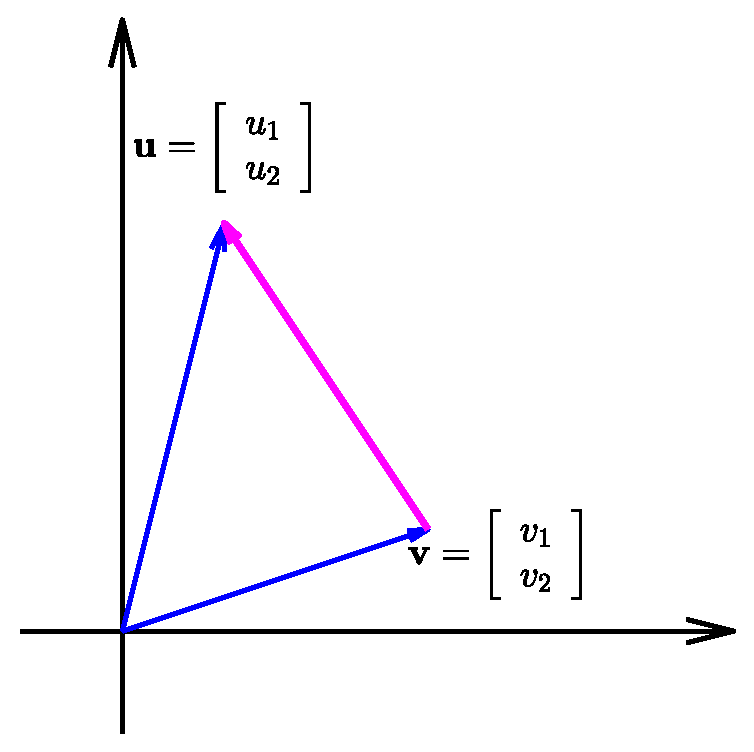
\includegraphics[width=4cm]{figures/UminusV} & \hspace*{12pt} &
	% \includegraphics[width=4cm]{figures/VminusU}
    % \end{tabular}
    \begin{center}
        \begin{tikzpicture}[scale=1, transform shape]
        \tikzset{>=latex}
	\coordinate (P) at (0.6,2);
        \coordinate (Q) at (1.9,0.5);
        \coordinate (0) at (0,0);
        \draw [->] (-0.2,0) -- (2.5,0);
        \draw [->] (0,-0.2) -- (0,2.5);
	\draw [->] (0) -- (P) node [right] {$\vec{u}=\begin{pmatrix} u_1\cr u_2 \end{pmatrix}  $};
	\draw [->](0) -- (Q) node [right] {$\vec{v}=\begin{pmatrix} v_1\cr v_2 \end{pmatrix}  $};
	\draw [blue,<-,thick] (P) -- (Q);
    \end{tikzpicture}
    \end{center}
\end{center}
\end{frame}
%-------------- end slide -------------------------------%}}}
\section[\textcolor{yellow}{}]{\textcolor{yellow}{Parallel Vectors}}
%-------------- start slide -------------------------------%{{{ 11
\begin{frame}
\frametitle{Parallel Vectors}
\pause
\begin{definition}
    Two vectors are called \alert{parallel} if they lie on the same line. Equivalently, two vectors are parallel if they are scalar multiples of each other.
\end{definition}

\vspace{12pt}
\begin{example}

Determine if $\vec{v}$,  $\vec{w}$, $\vec{z}$ are parallel to
$
\vec{u} = \left[ \begin{array}{r} 3 \\ -2 \\ 1 \end{array} \right]
$
\begin{itemize}
    \item[]
	$
	\vec{v} = \left[ \begin{array}{r} 6 \\ -4 \\ 2 \end{array} \right]
	$
    \item[]
    \item[]
	$
	\vec{w} = \left[ \begin{array}{r} -6 \\ 4 \\ -2 \end{array} \right]
	$
    \item[]
    \item[]
	$
	\vec{z} = \left[ \begin{array}{r} 1 \\ 1 \\ 1 \end{array} \right]
	$
\end{itemize}
\end{example}
\end{frame}

%-------------- end slide -------------------------------%}}}
%-------------- start slide -------------------------------%{{{ 12
\begin{frame}[fragile]
    \begin{center}
	The following slides are for you to study by yourself\\[1em]
	as reviewing matereial...
    \end{center}
\end{frame}
%-------------- end slide -------------------------------%}}}
%-------------- start slide -------------------------------%{{{ 13
\frame{\frametitle{Scalar quantities versus vector quantities}
\begin{emptytitle}
    \begin{itemize}
	\item A \alert{scalar} quantity has only magnitude; e.g.\ time, temperature.
	\pause
	\item A \alert{vector} quantity has both magnitude and direction; e.g.\ displacement, force, wind velocity.
    \end{itemize}
    \pause
    Whereas two scalar quantities are equal if they are represented
    by the same value,
    two vector quantities are equal if and only if they have
    the same \alert{magnitude} and \alert{direction}.
\end{emptytitle}
}
%-------------- end slide -------------------------------%}}}
%-------------- start slide -------------------------------%{{{ 14
\frame{
\begin{alertblock}{$\RR^2$ and $\RR^3$}
    Vectors in $\RR^2$ and $\RR^3$ have convenient geometric
    representations as {\bf position vectors} of points in
    the 2-dimensional (Cartesian) plane and in 3-dimensional
    space, respectively.
\end{alertblock}
}
%-------------- end slide -------------------------------%}}}
%-------------- start slide -------------------------------%{{{ 15
\begin{frame}[fragile]
    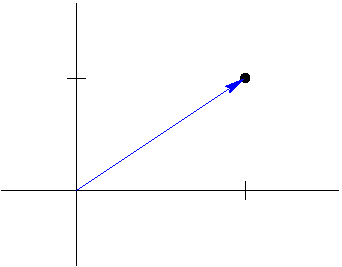
\includegraphics[scale=0.11]{R2.png}
    \hfill
    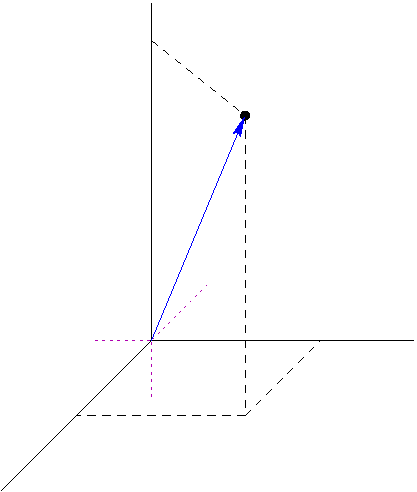
\includegraphics[scale=0.1]{R3.png}
\end{frame}
%-------------- end slide -------------------------------%}}}
%-----------------------start slide-----------------------%{{{ 16
\frame{
\begin{block}{Notation}
\begin{itemize}
    \item If $P$ is a point in $\mathbb{R}^3$ with coordinates $(x,y,x)$ we denote this by $P = (x,y,z)$.
    \pause
    \item If $P=(x,y,z)$ is a point in $\RR^3$, then
	\[\longvect{0P}=\left[\begin{array}{c}
	x \\ y\\ z \end{array}\right] \]
	is often used to
	denote the position vector of the point.
	\pause
    \item Instead of using a capital letter to denote the vector (as we generally do with matrices),
	we emphasize the importance of the geometry and the direction with an arrow over the name of the
	vector.
\end{itemize}
\end{block}
}
%-------------- end slide -------------------------------%}}}
%-------------- start slide -------------------------------%{{{ 17
\frame{
\begin{block}{Notation and Terminology}
    \begin{itemize}
	\item The notation $\longvect{0P}$ emphasizes that this vector goes from the origin $0$ to the point $P$. We can also use lower case letters for names of vectors. In this case, we write $\longvect{0P} = \vec{p}$.
	\pause
	\item Any vector
	    \[ \vec{x} =\left[\begin{array}{c} x_1 \\ x_2 \\ x_3\end{array}\right]
		\mbox{ in } \RR^3 \]
	    is associated with the \alert{point $(x_1, x_2, x_3)$}.
	\pause
	\item Often, \alert{there is no distinction made between the vector $\vec{x}$ and the point $(x_1, x_2,x_3)$},
	    \pause and we say that both \alert{$(x_1, x_2, x_3) \in \RR^3$ and $\vec{x} =\left[\begin{array}{c} x_1 \\ x_2
	    \\ x_3\end{array}\right] \in \mathbb{R}^3$.}
    \end{itemize}
\end{block}
}
%-------------- end slide -------------------------------%}}}
\section[\textcolor{yellow}{}]{\textcolor{yellow}{Length and Direction}}
%-------------- start slide -------------------------------%{{{ 18
\frame{
\frametitle{Length and Direction}
\pause
\begin{theorem}
    Let
    $\vec{v}=
    \left[\begin{array}{c}
    x \\ y\\ z \end{array}\right]$
    and
    $\vec{w}=
    \left[\begin{array}{c}
    x_1 \\ y_1\\ z_1 \end{array}\right]$
    be vectors in $\RR^3$.
    Then
    \begin{enumerate}
    \item<2->
    $\vec{v}=\vec{w}$ if and only if
    $x=x_1$, $y=y_1$, and $z=z_1$.
    \item<3->
    $||\vec{v}||=\sqrt{x^2+y^2+z^2}$.
    \item<4->
    $\vec{v}=\vec{0}$ if and only if
    $||\vec{v}||=0$.
    \item<5->
    For any scalar $a$,
    $||a\vec{v}|| =
    |a|\cdot ||\vec{v}||$.
    \end{enumerate}
\end{theorem}
\vfill

\uncover<6->{
\begin{remark}
Analogous results hold for $\vec{v}, \vec{w}\in\RR^2$, i.e.,
\[ \vec{v}=
\left[\begin{array}{c}
x \\ y \end{array}\right],
\vec{w}=
\left[\begin{array}{c}
x_1 \\ y_1 \end{array}\right].\]

In this case, $||\vec{v}||=\sqrt{x^2+y^2}$.}
    \end{remark}
}
%-------------- end slide -------------------------------%}}}
%-------------- start slide -------------------------------%{{{ 19
\frame{
\begin{example}
Let $\vec{p}=
\left[\begin{array}{c}
-3 \\ 4 \end{array}\right]$,
$\vec{q}=
\left[\begin{array}{c}
3 \\ -1 \\ -2 \end{array}\right]$,
and
$-2\vec{q}=
\left[\begin{array}{c}
-6 \\ 2 \\ 4 \end{array}\right]$,


\uncover<2->{
Then
\[ ||\vec{p}|| = \sqrt{(-3)^2 + 4^2} =\sqrt{9+16} = 5,\]}
\uncover<3->{
\[ ||\vec{q}|| = \sqrt{(3)^2 + (-1)^2 + (-2)^2}
=\sqrt{9+1 + 3} = \sqrt{14},\]}
\uncover<4->{
and
\begin{eqnarray*}
||-2\vec{q}|| & = & \sqrt{(-6)^2 + 2^2 + 4^2} \\
& = & \sqrt{36+4 + 16}\\
& = & \sqrt{56} = \sqrt{4\times 14}\\
& = & 2\sqrt{14} = 2||\vec{q}||.
\end{eqnarray*}
}
\end{example}
}
%-------------- end slide -------------------------------%}}}
\section[\textcolor{yellow}{}]{\textcolor{yellow}{Geometric Vectors}}
%-------------- start slide -------------------------------%{{{ 20
\frame{
\frametitle{Geometric Vectors}
\pause
Let $A$ and $B$ be two points in $\RR^2$ or $\RR^3$.
\begin{picture}(3,2.2)
    \put(0.1,0){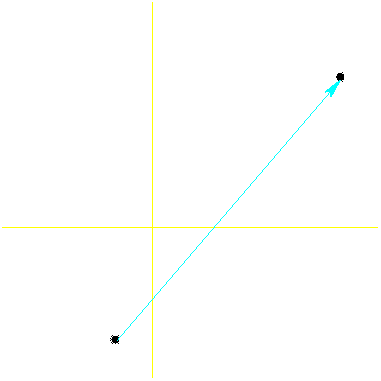
\includegraphics[scale=.75]{figures/vectors-1_copy.pdf}}
    \put(0.75,0.65){\small $0$}
    \put(1.8,0.65){\small $x$}
    \put(0.75,1.7){\small $y$}
    \put(1.65,1.5){\small $B$}
    \put(0.5,0.15){\small $A$}
    \put(2.2,1.5){\small $\bullet$ $\overrightarrow{AB}$ is the
    \alert{geometric vector} from $A$ to $B$.}
    \put(2.2,1.3){\small $\bullet$ $A$ is the \alert{tail} of
    $\overrightarrow{AB}$.}
    \put(2.2,1.1){\small $\bullet$ $B$ is the \alert{tip} of
    $\overrightarrow{AB}$.}
    \put(2.2,0.9){\small $\bullet$ the \alert{magnitude} of
    $\overrightarrow{AB}$ is its length, and is}
    \put(2.32,0.72){\small denoted $||\overrightarrow{AB}||$.}
\end{picture}
}
%-------------- end slide -------------------------------%}}}
%-------------- start slide -------------------------------%{{{ 21
\frame{
    \begin{picture}(3,2.2)
	\put(0.1,0){\includegraphics[scale=.75]{figures/vectors-2_copy.pdf}}
	\put(0.75,0.65){\small $0$}
	\put(2.1,0.65){\small $x$}
	\put(0.75,2.0){\small $y$}
	\put(1.3,0.60){\small $A$}
	\put(1.8,1.85){\small $B$}
	\put(0.15,0.15){\small $C$}
	\put(0.7,1.3){\small $D$}
	\put(2.3,1.6){\small $\bullet$ $\overrightarrow{AB}$ is the
	vector from $A(1,0)$ to $B(2,2)$.}
	\put(2.3,1.4){\small $\bullet$ $\overrightarrow{CD}$ is the
	vector from $C(-1,-1)$}
	\put(2.43,1.25){\small to $D(0,1)$.}
	\put(2.3,0.2){\small $\bullet$
	    $\overrightarrow{AB} = \overrightarrow{CD}$
	because the vectors have}
	\put(2.43,0.05){\small the same \alert{length}
	and \alert{direction}.}
    \end{picture}
}
%-------------- end slide -------------------------------%}}}
%-------------- start slide -------------------------------%{{{ 22
\frame{
    \begin{definition}
	A vector is in \alert{standard position} if its tail is at
	the origin.
    \end{definition}
    \medskip

    We co-ordinatize vectors by putting them in standard position,
    and then identifying them with their tips.

    \vspace*{-.2in}
    \begin{picture}(3,2)
	\put(1.1,0){\includegraphics[scale=.75]{figures/vectors-3_copy.pdf}}
	\put(1.35,0.25){\small $0$}
	\put(2.7,0.25){\small $x$}
	\put(1.35,1.6){\small $y$}
	\put(1.9,0.2){\small $A$}
	\put(2.65,1.45){\small $B$}
	\put(1.9,1.45){\small $P$}
    \end{picture}

    Thus $\overrightarrow{AB}=\overrightarrow{0P}$ where
    $P=P(1,2)$, and we write
    $\overrightarrow{0P}=
    \left[\begin{array}{c}
    1 \\ 2 \end{array}\right]=\overrightarrow{AB}$.

    $\overrightarrow{0P}$ is the \alert{position vector} for
    $P(1,2)$.
}
%-------------- end slide -------------------------------%}}}
%-------------- start slide -------------------------------%{{{ 23
\frame{
\begin{emptytitle}
  More generally, if $P(x,y,z)$ is a point in $\RR^3$, then
$\overrightarrow{0P}=
\left[\begin{array}{c}
x \\ y\\ z \end{array}\right]$
is the position vector for $P$.
\bigskip

\uncover<2->{
If we aren't concerned with the locations of the tail and
tip, we simply write
$\vec{v}=
\left[\begin{array}{c}
x \\ y\\ z \end{array}\right]$}
\end{emptytitle}
}
%-------------- end slide -------------------------------%}}}
\section[\textcolor{yellow}{}]{\textcolor{yellow}{The Parallelogram Law}}
%-------------- start slide -------------------------------%{{{ 24
\frame{
    \frametitle{Intrinsic Description of Vectors}
    \pause
    \begin{itemize}
	\item<2->
	    \alert{vector equality}: same length and direction.
	    \vfill
	\item<3->
	    \alert{$\vec{0}$}: the vector with length zero and
	    \alert{no direction}.
	    \vfill
	\item<4->
	    \alert{scalar multiplication}:
	    if $\vec{v}\neq\vec{0}$ and $a\in\RR$, $a\neq 0$,
	    then $a\vec{v}$ has length $|a|\cdot ||\vec{v}||$ and
	    \begin{itemize}
		\normalsize
	    \item the same direction as $\vec{v}$ if $a>0$;
	    \item direction opposite to $\vec{v}$ if $a<0$.
	\end{itemize}
	\vfill
    \item<5->
	\alert{addition}: $\vec{u}+\vec{v}$ is the diagonal of
	the parallelogram defined by $\vec{u}$ and $\vec{v}$,
	and having the same tail as $\vec{u}$ and $\vec{v}$.
\end{itemize}

\uncover<6->{
    \begin{picture}(3.5,1.2)
	\put(1.4,0){\includegraphics[scale=1]{figures/vectors-4_copy.pdf}}
	\put(1.5,0.3){$\vec{u}$}
	\put(1.95,0.6){$\vec{u}+\vec{v}$}
	\put(2.6,0.0){$\vec{v}$}
    \end{picture}
    \begin{center}
	parallelogram law
\end{center}}
}
%-------------- end slide -------------------------------%}}}
%-------------- start slide -------------------------------%{{{ 25
\frame{
If we have a coordinate system, then
\begin{itemize}
    \item<2-> \alert{vector equality}: $\vec{u}=\vec{v}$ if and only if $\vec{u}$ and $\vec{v}$ are equal as matrices.
    \item<3-> \alert{$\vec{0}$}: has all coordinates equal to zero.
    \item<4-> \alert{scalar multiplication}: $a\vec{v}$ is obtained from $\vec{v}$ by multiplying each entry of $\vec{v}$ by $a$ (matrix scalar multiplication).
    \item<5-> \alert{addition}: $\vec{u}+\vec{v}$ is represented by the matrix sum of the columns $\vec{u}$ and $\vec{v}$.
\end{itemize}
}
%-------------- end slide -------------------------------%}}}
%-------------- start slide -------------------------------%{{{ 26
\frame{
    \frametitle{Tip-to-Tail Method for Vector Addition}
    For points $A$, $B$ and $C$,
    \[ \overrightarrow{AB} + \overrightarrow{BC}
    =\overrightarrow{AC}.\]
    \bigskip

    \begin{picture}(3.5,1.2)
	\put(1.4,0){\includegraphics[scale=1]{figures/vectors-5_copy.pdf}}
	\put(1.8,-0.1){\small $A$}
	\put(3.25,0.25){\small $B$}
	\put(2.65,1.15){\small $C$}
	\put(2.5,-0.1){\small$\overrightarrow{AB}$}
	\put(3.0,0.6){\small$\overrightarrow{BC}$}
	\put(2.05,0.6){\small$\overrightarrow{AC}$}
	\put(1.9,1.0){\tiny$\overrightarrow{AB}$}
	\put(1.5,0.25){\tiny$\overrightarrow{BC}$}
    \end{picture}
}
%-------------- end slide -------------------------------%}}}
%-------------- start slide -------------------------------%{{{ 27
\frame{
    \begin{problem}
    % \textcolor{titleDarkBlue}{Example}\\[0.5em]
    Show that the diagonals of any parallelogram bisect each other.
    \end{problem}
    \vfill
    \pause
   \begin{proofnoend}

	Denote the parallelogram by its vertices, $ABCD$.

	\begin{picture}(2.5,1.3)
	    \put(0.2,0.2){\includegraphics[scale=1]{figures/vectors-6_copy.pdf}}
	    % \put(0.2,0.2){\includegraphics[scale=1]{figures/vectors-6.pdf}}
	    \put(0.1,0.1){\small{$A$}}
	    \put(0.55,1){\small{$B$}}
	    \put(2.05,1){\small{$C$}}
	    \put(1.5,0.1){\small{$D$}}
	    \put(0.9,0.6){\tiny{$M$}}
	    \put(2.5,.9){$\bullet$ Let $M$ denote the midpoint}
	    \put(2.65,.7){of $\overrightarrow{AC}$.}
	    \put(2.65,.5){Then $\overrightarrow{AM}=\overrightarrow{MC}$.}
	    \put(2.5,.3){$\bullet$ It now suffices to show}
	    \put(2.65,.1){that $\overrightarrow{BM}=\overrightarrow{MD}$.}
    \end{picture}

   \bigskip
   \pause

    \[ \overrightarrow{BM}
	    = \overrightarrow{BA} +\overrightarrow{AM}
	    = \overrightarrow{CD} +\overrightarrow{MC}
	    = \overrightarrow{MC} +\overrightarrow{CD}
    = \overrightarrow{MD}.\]

   \bigskip
   \pause

    Since $\overrightarrow{BM}=\overrightarrow{MD}$, these
    vectors have the same \alert{magnitude} and \alert{direction},
    implying that $M$ is the midpoint of $\overrightarrow{BD}$.
   \bigskip
   \pause


    Therefore, the diagonals of $ABCD$ bisect each other.
\myQED   \end{proofnoend}
}
%-------------- end slide -------------------------------%}}}
%-------------- start slide -------------------------------%{{{ 28
\frame{\frametitle{Vector Subtraction}
    \begin{itemize}
	\item<2->
	    If we have a coordinate system, then subtract the vectors as you
	    would subtract matrices.
	    \vfill
	\item<3->
	    For the intrinsic description:

	    \begin{picture}(2.5,1.0)
		\put(1.2,0){\includegraphics[scale=1]{figures/vectors-7_copy.pdf}}
		\put(1.2,0.4){\small{$\vec{v}$}}
		\put(1.65,-0.1){\small{$\vec{u}$}}
		\put(1.9,0.85){\small{$\vec{u}$}}
		\put(2.4,0.4){\small{$-\vec{v}$}}
		\put(1.9,0.4){\small{$\vec{u}-\vec{v}$}}
	    \end{picture}
	    \bigskip

	    $\vec{u}-\vec{v} = \vec{u} + (-\vec{v})$
	    and is the diagonal from the tip of $\vec{v}$ to the
	    tip of $\vec{u}$ in the parallelogram defined by
	    $\vec{u}$ and $\vec{v}$.
    \end{itemize}
}
%-------------- end slide -------------------------------%}}}
%-------------- start slide -------------------------------%{{{ 29
\frame{
    \begin{theorem}
	Let $P_1(x_1,y_1,z_1)$ and $P_2(x_2,y_2,z_2)$ be two
	points.  Then
	\begin{enumerate}
	    \item<2->
		\[ \overrightarrow{P_1P_2} =
		    \left[\begin{array}{c}
			    x_2 - x_1 \\
			    y_2 - y_1 \\
			    z_2 - z_1
		    \end{array}\right].\]
		\item<3->
		    The distance between $P_1$ and $P_2$ is
		    \[ \sqrt{(x_2-x_1)^2 + (y_2-y_1)^2 +(z_2-z_1)^2}.\]
		    \vspace*{-0.2in}

	    \end{enumerate}
	\end{theorem}

	\uncover<4->{
	    \begin{proofnoend}
		\begin{center}
		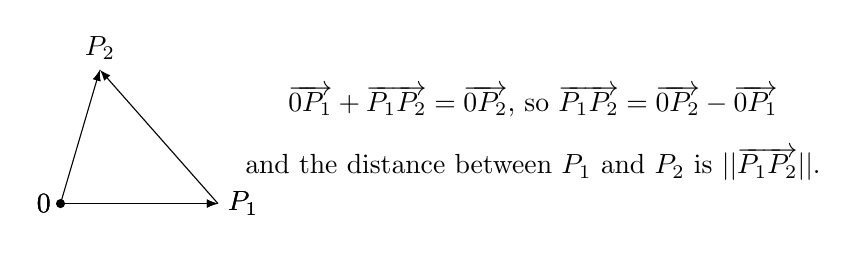
\begin{tikzpicture}[scale=1, transform shape]
		    \tikzset{>=latex}
		    \draw [->] (0,0) node [left] {0}-- (2,0) node [right] {$P_1$};
		    \draw [->] (0,0) node [left] {0}-- (2,0) node [right] {$P_1$};
		    \draw [->] (0,0) node [left] {0}-- (0.5,1.7) node [above] {$P_2$};
		    \draw [->] (2,0) -- (0.5,1.7);
		    \filldraw (0,0) circle (0.05);
		    \node at (6,1.3) {$\overrightarrow{0P_1} + \overrightarrow{P_1P_2}
			=\overrightarrow{0P_2}$, so
			$\overrightarrow{P_1P_2} = \overrightarrow{0P_2}
		    -\overrightarrow{0P_1}$};
		    \node at (6, 0.5) {and the distance between $P_1$ and $P_2$ is
		    $||\overrightarrow{P_1P_2}||$.};
		\end{tikzpicture}
		\end{center}
		% \begin{picture}(2.5,0.9)
		% \put(0.25,0.1){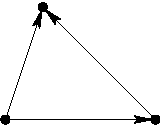
\includegraphics[scale=1]{figures/vectors-8.pdf}}
		% \put(0.15,0){\small $0$}
		% \put(1.35,0){\small $P_1$}
		% \put(0.63,0.85){\small $P_2$}
		% \put(1.6,0.8){
		% $\overrightarrow{0P_1} + \overrightarrow{P_1P_2}
		% =\overrightarrow{0P_2}$, so
		% $\overrightarrow{P_1P_2} = \overrightarrow{0P_2}
		% -\overrightarrow{0P_1}$,}
		% \put(1.6,0.55){
		% and the distance between $P_1$ and $P_2$ is
		% $||\overrightarrow{P_1P_2}||$.}
		% \end{picture}
\myQED	\end{proofnoend}}
    }
%-------------- end slide -------------------------------%}}}
%-------------- start slide -------------------------------%{{{ 30
\frame{
\begin{example}
For $P(1,-1,3)$ and $Q(3,1,0)$
\[
\overrightarrow{PQ} =
\left[\begin{array}{c}
3-1\\1-(-1)\\0-3
\end{array}\right]
=
\left[\begin{array}{r}
2\\2\\-3
\end{array}\right]\]
and the distance between $P$ and $Q$ is
$||\overrightarrow{PQ}||= \sqrt{2^2 + 2^2 + (-3)^2}
=\sqrt{17}$.
\end{example}

\uncover<2->{
\begin{definition}
A \alert{unit vector} is a vector of length one.
\end{definition}}

\uncover<3->{
\begin{example}
$\left[\begin{array}{c}
1 \\ 0 \\ 0
\end{array}\right]$,
$\left[\begin{array}{c}
0 \\ 1 \\ 0
\end{array}\right]$,
$\left[\begin{array}{c}
0 \\ 0 \\ 1
\end{array}\right]$,
$\left[\begin{array}{c}
\frac{\sqrt{2}}{2} \\ 0 \\ \frac{\sqrt{2}}{2}
\end{array}\right]$,
are examples of unit vectors.
\end{example}}
}
%-------------- end slide -------------------------------%}}}
%-------------- start slide -------------------------------%{{{ 31
\frame{
\begin{example}
$\vec{v}=\left[\begin{array}{r}
-1 \\ 3 \\ 2
\end{array}\right]$
is not a unit vector, since $||\vec{v}||=\sqrt{14}$.
\uncover<2->{
However,
\[ \vec{u}=\frac{1}{\sqrt{14}}\vec{v}
=\left[\begin{array}{c}\vspace*{.02in}
\frac{-1}{\sqrt{14}} \\ \vspace*{.02in}
\frac{3}{\sqrt{14}} \\
\frac{2}{\sqrt{14}} \end{array}\right]\]
is a unit vector \alert{in the same direction} as $\vec{v}$,}
\uncover<3->{
i.e.,
\[ ||\vec{u}|| =
\frac{1}{\sqrt{14}} ||\vec{v}||
=\frac{1}{\sqrt{14}} \sqrt{14}=1.\]}
\end{example}
}
%-------------- end slide -------------------------------%}}}
%-------------- start slide -------------------------------%{{{ 32
\frame{
\begin{example}
If $\vec{v}\neq\vec{0}$, then
\[ \frac{1}{||\vec{v}||} \vec{v} \]
is a unit vector in the same direction as $\vec{v}$.
\end{example}
}
%-------------- end slide -------------------------------%}}}
%-------------- start slide -------------------------------%{{{ 33
\frame{
    % \begin{example}
    % \textcolor{titletextcolour}{Example}\\[0.5em]
    \begin{problem}
    Find the point, $M$, that is midway between $P_1(-1,-4,3)$
    and $P_2(5,0,-3)$.
    \end{problem}
    % \begin{picture}(2.5,1.4)
    %     \put(1.5,0.1){\includegraphics[scale=.8]{figures/vectors-9.pdf}}
    %     \put(1.4,0){\small $0$}
    %     \put(1.5,1.1){\small $P_1$}
    %     \put(2.25,1.0){\small $M$}
    %     \put(3.0,0.65){\small $P_2$}
    % \end{picture}
    \begin{center}
	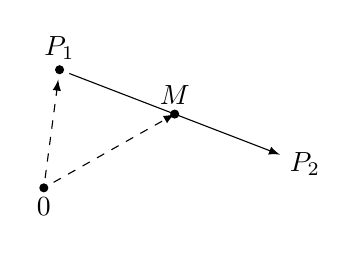
\begin{tikzpicture}[scale=1, transform shape]
	    \tikzset{>=latex}
	    \node (0) at (0,0) {};
	    \node (1) at (0.2,1.5) {};
	    \node (2) at (3,0.3) [right] {$P_2$};
	    \draw [->] (1) -- coordinate[midway,above] (m) (2);
	    \draw [->,dashed] (0) node [below] {$0$} -- (1) node [above] {$P_1$};
	    \draw [->,dashed] (0) -- (m) node [above] {$M$};
	    \filldraw (m) circle (0.05);
	    \filldraw (0) circle (0.05);
	    \filldraw (1) circle (0.05);
	    % \draw [->,dashed] (0,0) -- (0.5,1) node [above] {$M$};
	    % \draw []
	    % \draw [->] (0,0) node [left] {0}-- (0.5,1.7) node [above] {$P_2$};
	    % \draw [->] (2,0) -- (0.5,1.7);
	    % \filldraw (0,0) circle (0.05);
	    % \node at (6,1.3) {$\overrightarrow{0P_1} + \overrightarrow{P_1P_2}
	    % =\overrightarrow{0P_2}$, so
	    % $\overrightarrow{P_1P_2} = \overrightarrow{0P_2}
	    % -\overrightarrow{0P_1}$};
	    % \node at (6, 0.5) {and the distance between $P_1$ and $P_2$ is
	    % $||\overrightarrow{P_1P_2}||$.};
	\end{tikzpicture}
    \end{center}
\vfill \pause
\begin{solution}
    \begin{eqnarray*}
	\overrightarrow{0M}
	= \overrightarrow{0P_1}
	+ \overrightarrow{P_1M}
	=\overrightarrow{0P_1}
	+\frac{1}{2} \overrightarrow{P_1P_2}
& = &
\left[\begin{array}{r}
	-1 \\ -4 \\ 3
\end{array}\right]
+ \frac{1}{2}
\left[\begin{array}{r}
	6 \\ 4 \\ -6
\end{array}\right] \\
& = &
\left[\begin{array}{r}
	-1 \\ -4 \\ 3
\end{array}\right]
+
\left[\begin{array}{r}
	3 \\ 2 \\ -3
\end{array}\right]
=
\left[\begin{array}{r}
	2 \\ -2 \\ 0
\end{array}\right].
    \end{eqnarray*}

    Therefore, $M=M(2,-2,0)$.
\end{solution}
}
%-------------- end slide -------------------------------%}}}
%-------------- start slide -------------------------------%{{{ 34
\frame{
    \begin{problem}
    Find the two points trisecting the segment between $P(2,3,5)$
    and $Q(8,-6,2)$.
    % \begin{picture}(2.5,1.1)
    % \put(1.5,0.1){\includegraphics[scale=.7]{figures/vectors-10.pdf}}
    % % \put(1.5,0.1){\includegraphics[scale=.7]{figures/output.pdf}}
    % % \put(1.5,0.1){\includegraphics[scale=.7]{figures/inverted.pdf}}
    % \put(1.8,0){\small $0$}
    % \put(1.4,1){\small $P$}
    % \put(1.85,0.9){\small $A$}
    % \put(2.2,0.75){\small $B$}
    % \put(2.6,0.4){\small $Q$}
    % \end{picture}
    \begin{center}
	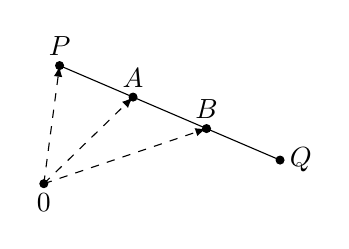
\begin{tikzpicture}[scale=1, transform shape]
	    \tikzset{>=latex}
	    \coordinate (P) at (0.2,1.5);
	    \coordinate (Q) at (3,0.3);
	    \coordinate (0) at (0,0);
	    \draw (P) -- coordinate[pos={1/3}] (A) coordinate[pos={2/3}] (B) (Q) node [right] {$Q$};
	    \draw [->,dashed] (0) node [below] {$0$} -- (P) node [above] {$P$};
	    \draw [->,dashed] (0) -- (A) node [above] {$A$};
	    \draw [->,dashed] (0) -- (B) node [above] {$B$};
	    \filldraw (P) circle (0.05);
	    \filldraw (Q) circle (0.05);
	    \filldraw (0) circle (0.05);
	    \filldraw (A) circle (0.05);
	    \filldraw (B) circle (0.05);
	\end{tikzpicture}
    \end{center}
\end{problem}
\vfill \pause
\begin{solution}
    $\overrightarrow{0A}
    = \overrightarrow{0P} + \frac{1}{3} \overrightarrow{PQ}$
    and
    $\overrightarrow{0B}
    = \overrightarrow{0P} + \frac{2}{3} \overrightarrow{PQ}$.
    \uncover<3->{\small
	Since $\overrightarrow{PQ}=
	\left[\begin{array}{r}
		6 \\ -9 \\ -3
	\end{array}\right]$,
	$\overrightarrow{0A}=
	\left[\begin{array}{r}
		2 \\ 3 \\ 5
	\end{array}\right]
	+
	\left[\begin{array}{r}
		2 \\ -3 \\ -1
	\end{array}\right]
	=\left[\begin{array}{r}
		4 \\ 0 \\ 4
	\end{array}\right]$, and
	$\overrightarrow{0B}=
	\left[\begin{array}{r}
		2 \\ 3 \\ 5
	\end{array}\right]
	+
	\left[\begin{array}{r}
		4 \\ -6 \\ -2
	\end{array}\right]
	=\left[\begin{array}{r}
		6 \\ -3 \\ 3
    \end{array}\right]$.  }
    \bigskip

    \uncover<4->{
    Therefore, the two points are $A(4,0,4)$ and $B(6,-3,3)$.}
\end{solution}
}
%-------------- end slide -------------------------------%}}}
%-------------- start slide -------------------------------%{{{ 35
\frame{
    \begin{problem}
    % \textcolor{titletextcolour}{Example}\\[0.5em]
    Let $ABCD$ be an arbitrary quadrilateral.
    Show that the midpoints of the four sides of $ABCD$ are the
    vertices of a parallelogram.
    \end{problem}
    \pause

    \begin{proofnoend}
    \begin{picture}(2.5,1.4)
	\put(0.2,0.1){\includegraphics[scale=0.9]{figures/vectors-11_copy.pdf}}
	\put(0.05,0.75){\small $A$}
	\put(0.5,1.2){\small $B$}
	\put(1.85,0.55){\small $C$}
	\put(0.7,0){\small $D$}
	\put(2.2,1.1){\small Let $M_1$ denote the
	midpoint of $\overrightarrow{AB}$,}
	\put(2.43,0.9){\small $M_2$ the midpoint of $\overrightarrow{BC}$,}
	\put(2.43,0.7){\small $M_3$ the midpoint of $\overrightarrow{CD}$, and}
	\put(2.43,0.5){\small $M_4$ the midpoint of $\overrightarrow{DA}$.}
	\put(0.3,1.05){\tiny $M_1$}
	\put(1.25,1.0){\tiny $M_2$}
	\put(1.35,0.25){\tiny $M_3$}
	\put(0.4,0.35){\tiny $M_4$}
    \end{picture}

    We need to prove that
    $\overrightarrow{M_1M_2} = \overrightarrow{M_4M_3}$ and
    $\overrightarrow{M_1M_4} = \overrightarrow{M_2M_3}$.
    \end{proofnoend}
}
%-------------- end slide -------------------------------%}}}
%-------------- start slide -------------------------------%{{{ 36
\begin{frame}[fragile]
    \begin{proofnoend}[continued]
       We will show $\overrightarrow{M_1M_4} = \overrightarrow{M_2M_3}$, the other relation can be shown in the same way.
       \pause\vspace{1em}
       Notice that
       \begin{align*}
	   \overrightarrow{0M_1} =  \overrightarrow{0A} + \frac{1}{2} \overrightarrow{AB} &&
	   \overrightarrow{0M_2} =  \overrightarrow{0C} + \frac{1}{2} \overrightarrow{CB} \\
	   \overrightarrow{0M_4} =  \overrightarrow{0A} + \frac{1}{2} \overrightarrow{AD} &&
	   \overrightarrow{0M_3} =  \overrightarrow{0C} + \frac{1}{2} \overrightarrow{CD}
       \end{align*}
       \pause
       Hence,
       \begin{align*}
	   \overrightarrow{M_1M_4} =  \overrightarrow{0M_4} - \overrightarrow{0M_1} = \frac{1}{2} \left(\overrightarrow{AD} - \overrightarrow{AB}\right)= \frac{1}{2}\overrightarrow{BD}
       \end{align*}
	and
       \begin{align*}
	   \overrightarrow{M_2M_3} =  \overrightarrow{0M_3} - \overrightarrow{0M_2} = \frac{1}{2} \left(\overrightarrow{CD} - \overrightarrow{CB}\right) = \frac{1}{2}\overrightarrow{BD}
       \end{align*}
       \pause\vspace{1em}
	Therefore, $\overrightarrow{M_1M_4} = \overrightarrow{M_2M_3}$.
    \myQED\end{proofnoend}
\end{frame}
%-------------- end slide -------------------------------%}}}
%-------------- start slide -------------------------------%{{{ 37
\frame{

\begin{definition}
    Two nonzero vectors are called \alert{parallel} if and only if
    they have the same direction or opposite directions.
\end{definition}
\vfill
\pause

\begin{theorem}
    Two nonzero vectors $\vec{v}$ and $\vec{w}$ are parallel if and only
    if one is a scalar multiple of the other.
\end{theorem}
\vfill
\pause

\begin{emptytitle}
    In particular, if $\vec{v}$ and $\vec{w}$ are nonzero and have the
    same direction, then
    $\vec{v}=\frac{||\vec{v}||}{||\vec{w}||}\vec{w}$;
    if $\vec{v}$ and $\vec{w}$ have opposite directions, then
    $\vec{v}=-\frac{||\vec{v}||}{||\vec{w}||}\vec{w}$.
\end{emptytitle}
}
%-------------- end slide -------------------------------%}}}
\section[\textcolor{yellow}{}]{\textcolor{yellow}{Lines in Space}}
%-------------- start slide -------------------------------%{{{ 38
\frame{
    \frametitle{Equations of lines}
    \pause
    Let $L$ be a line, $P_0(x_0,y_0,z_0)$ a fixed point on $L$,
    $P(x,y,z)$ an arbitrary point on $L$, and
    $\vec{d}
    =\left[\begin{array}{c}
	    a \\ b \\ c
    \end{array}\right]$ a \alert{direction vector} for $L$,
    i.e., a vector parallel to $L$.

    % \begin{picture}(3.5,0.6)
    % \put(3.2,0.1){\includegraphics[scale=.7]{figures/vectors-12.pdf}}
    % \put(3.1,0.4){\small $L$}
    % \put(3.4,0.1){\small $0$}
    % \put(3.4,0.62){\small $P_0$}
    % \put(4.3,0.60){\small $P$}
    % \put(3.8,0.7){\small $\vec{d}$}
    % \put(0,0.3){\small Then
    % $\overrightarrow{0P} =
    % \overrightarrow{0P_0} +\overrightarrow{P_0P}$, and
    % $\overrightarrow{P_0P}$ is parallel}
    % \put(0,0.1){to $\vec{d}$, so $\overrightarrow{P_0P}
    % =t\vec{d}$ for some $t\in\RR$.}
    % \end{picture}

    \begin{center}
	\begin{tikzpicture}[scale=1, transform shape]
	    \tikzset{>=latex}
	    \coordinate (L) at (3.1,0.4);
	    \coordinate (P0) at (0.2,1.2);
	    \coordinate (0) at (0,0);
	    \coordinate (P) at (3,2);
	    \draw ($(P)!-0.6cm!(P0)$)  -- (P) node [below]  {$P$} -- (P0) node [above] {$P_0$} -- ($(P0)!-0.6cm!(P)$) node [left] {$L$};
	    \draw [thick,->,color=blue] (P0) --coordinate [pos={1/2}] (m) node [above] {${\vec{d}}$} ($(P)!1cm!(P0)$);
	    \draw[dashed,->] (0) node [below] {$0$} -- (P0);
	    \draw[dashed,->] (0) -- (P);
	    \filldraw (P) circle (0.05);
	    \filldraw (P0) circle (0.05);
	    \filldraw (0) circle (0.05);
	    \node at ( -4,1 ) {Then $\overrightarrow{0P} = \overrightarrow{0P_0} +\overrightarrow{P_0P}$, and $\overrightarrow{P_0P}$ is parallel};
	    \node at (-4,0.2) {to $\vec{d}$, so $\overrightarrow{P_0P} =t\vec{d}$ for some $t\in\RR$.};
	\end{tikzpicture}
    \end{center}

    \pause \vfill 

    \begin{definition}
	Vector Equation of a Line: $\boxed{\overrightarrow{0P} = \overrightarrow{0P_0} + t\: \vec{d},\quad t\in\RR.}$
    \end{definition}
    \pause \vfill 
   \begin{remark}
	Notation in the text: $\vec{p}=\overrightarrow{0P}$,
	$\vec{p}_0=\overrightarrow{0P_0}$, so
	$\vec{p}=\vec{p}_0+t\vec{d}$.
   \end{remark}
}
%-------------- end slide -------------------------------%}}}
%-------------- start slide -------------------------------%{{{ 39
\frame{
    \begin{emptytitle}
	In component form, this is written as
	\[
	\left[\begin{array}{c}
	    x \\ y \\ z
	\end{array}\right]
	=
	\left[\begin{array}{c}
	    x_0 \\ y_0 \\ z_0
	\end{array}\right]
	+
	t \left[\begin{array}{c}
	    a \\ b \\ c
	\end{array}\right], t\in\RR.
	\]
    \end{emptytitle}

    \vfill
    \pause
    \begin{emptytitle}{\bf Parametric Equations of a Line}
	\[
	\begin{array}{rcl}
	    x & = & x_0 + ta \\
	    y & = & y_0 + tb \\
	    z & = & z_0 + tc
	\end{array},~~ t\in\RR.
	\]
    \end{emptytitle}
}
%-------------- end slide -------------------------------%}}}
%-------------- start slide -------------------------------%{{{ 40
\frame{
\begin{problem}
    Find an equation for the line through two points $P(2,-1,7)$ and
    $Q(-3,4,5)$.
\end{problem}
\vfill
\pause
\begin{solution}
    A direction vector for this line is
    \[ \vec{d}=\overrightarrow{PQ}=
    \left[\begin{array}{r}
    -5 \\ 5 \\ -2
    \end{array}\right].\]
    \pause
    \bigskip
    Therefore, a vector equation of this line is
    \[
    \left[\begin{array}{r}
    x \\ y \\ z
    \end{array}\right]
    =
    \left[\begin{array}{r}
    2 \\ -1 \\ 7
    \end{array}\right]
    +
    t \left[\begin{array}{r}
    -5 \\ 5 \\ -2
    \end{array}\right].
    \]
\end{solution}
}
%-------------- end slide -------------------------------%}}}
%-------------- start slide -------------------------------%{{{ 41
\frame{
\begin{problem}
    Find an equation for the line through $Q(4,-7,1)$ and parallel
    to the line
    \[ L:
    \left[\begin{array}{r}
    x \\ y \\ z
    \end{array}\right]
    =
    \left[\begin{array}{r}
    1 \\ -1 \\ 1
    \end{array}\right]
    +
    t \left[\begin{array}{r}
    2 \\ -5 \\ 3
    \end{array}\right]. \]
\end{problem}
\vfill
\pause
\begin{solution}
    The line has equation
    \[
    \left[\begin{array}{r}
    x \\ y \\ z
    \end{array}\right]
    =
    \left[\begin{array}{r}
    4 \\ -7 \\ 1
    \end{array}\right]
    +
    t \left[\begin{array}{r}
    2 \\ -5 \\ 3
    \end{array}\right], t\in\RR. \]
\end{solution}
}
%-------------- end slide -------------------------------%}}}
%-------------- start slide -------------------------------%{{{ 42
\frame{
\begin{problem}
Given two lines $L_1$ and $L_2$, find the point of intersection,
if it exists.
\[ L_1:
\begin{array}{rcl}
x & = & 3+t \\
y & = & 1-2t \\
z & = & 3+3t
\end{array}
\hspace*{1in}
L_2:
\begin{array}{rcl}
x & = & 4+2s \\
y & = & 6+3s \\
z & = & 1+s
\end{array}\]
\end{problem}
\vfill
\pause

\begin{solution}

Lines $L_1$ and $L_2$ intersect if and only if there are values
$s,t\in\RR$ such that
\[ \begin{array}{rcl}
3+t & = & 4 + 2s \\
1-2t & = & 6 + 3s \\
3 + 3t & = & 1 + s
\end{array}\]
\pause
i.e., if and only if the system
\[ \begin{array}{rcl}
2s-t & = & -1 \\
3s + 2t & = & -5 \\
s - 3t & = & 2
\end{array}\]
is consistent.
\end{solution}
}
%-------------- end slide -------------------------------%}}}
%-------------- start slide -------------------------------%{{{ 43
\frame{
\begin{solution}[continued]
\[
\left[\begin{array}{rr|r}
2 & -1 & -1 \\
3 & 2 & -5 \\
1 & -3 & 2
\end{array}\right]
\rightarrow \cdots \rightarrow
\left[\begin{array}{rr|r}
1 & 0 & -1 \\
0 & 1 & -1 \\
0 & 0 & 0
\end{array}\right]\]

\uncover<2->{
$L_1$ and $L_2$ intersect when $s=-1$ and $t=-1$.}
\bigskip

\uncover<3->{Using the
equation for $L_1$ and setting $t=-1$, the point of
intersection is
\[ P(3+(-1), 1-2(-1), 3+3(-1)) = P(2,3,0).\]}
\bigskip

\uncover<4->{
{\bf Note.} You can check your work by setting $s=-1$
in the equation for $L_2$.}
\end{solution}
}
%-------------- end slide -------------------------------%}}}
%-------------- start slide -------------------------------%{{{ 44
\frame{
    \begin{problem}
	% \textcolor{titletextcolour}{Example (continued)}\\[0.5em]
	Find equation{\bf s} for the lines through $P(1,0,1)$ that
	meet the line
	\[ L:
	    \left[\begin{array}{r}
		    x \\ y \\ z
	    \end{array}\right]
	    =
	    \left[\begin{array}{r}
		    1 \\ 2 \\ 0
	    \end{array}\right]
	    +
	    t \left[\begin{array}{r}
		    2 \\ -1 \\ 2
	    \end{array}\right]
	\]
	at points distance three from $P_0(1,2,0)$.
	\bigskip
	\begin{picture}(3.5,1.0)
	    \put(1.4,0.1){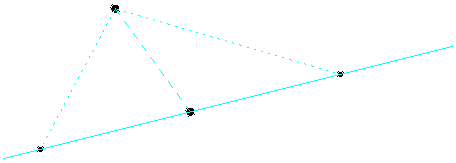
\includegraphics[scale=.7]{figures/vectors-13_copy.pdf}}
	    \put(1.4,0.2){\small $Q_1$}
	    \put(2.3,0.2){\small $P_0$}
	    \put(2.92,0.35){\small $Q_2$}
	    \put(1.8,0.8){\small $P$}
	\end{picture}
    \end{problem}
    \pause
    \begin{solution}
	Find points $Q_1$ and $Q_2$ on $L$ that are distance three
	from $P_0$, and then find equations for the lines through
	$P$ and $Q_1$, and through $P$ and $Q_2$.
    \end{solution}
	}
%-------------- end slide -------------------------------%}}}
%-------------- start slide -------------------------------%{{{ 45
\frame{
    \begin{solution}[continued]
	% \textcolor{titletextcolour}{Example (continued)}\\[0.5em]
	\begin{picture}(3.5,1.0)
	    \put(0.4,0.1){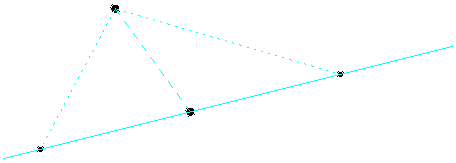
\includegraphics[scale=.7]{figures/vectors-13_copy.pdf}}
	    \put(0.4,0.2){\small $Q_1$}
	    \put(1.1,0.1){\small $P_0(1,2,0)$}
	    \put(1.92,0.35){\small $Q_2$}
	    \put(0.7,0.9){\small $P(1,0,1)$}
	    \put(3.0,.5){\small
	    $\vec{d}=\left[\begin{array}{r} 2 \\ -1 \\ 2\end{array}\right]$}
	\end{picture}
	\bigskip

	\uncover<2->{
	    First, $||\vec{d}||=\sqrt{2^2 + (-1)^2 +2^2}=\sqrt{9}=3$,
	    so
	    \[ \overrightarrow{0Q}_1=\overrightarrow{0P_0} +1\vec{d},
		\quad\text{and}\quad
	\overrightarrow{0Q}_2=\overrightarrow{0P_0} -1\vec{d}.\]}

	\uncover<3->{\small
	    \[
		\overrightarrow{0Q}_1 =
		\left[\begin{array}{r} 1 \\ 2 \\ 0\end{array}\right] +
		\left[\begin{array}{r} 2 \\ -1 \\ 2\end{array}\right]
		=
		\left[\begin{array}{r} 3 \\ 1 \\ 2\end{array}\right]
		\quad\text{and}\quad
		\overrightarrow{0Q}_2 =
		\left[\begin{array}{r} 1 \\ 2 \\ 0\end{array}\right] -
		\left[\begin{array}{r} 2 \\ -1 \\ 2\end{array}\right]
		=
		\left[\begin{array}{r} -1 \\ 3 \\ -2\end{array}\right],
	    \]
	so $Q_1 = Q_1(3,1,2)$ and $Q_2=Q_2(-1,3,-2)$.}
    \end{solution}
}
%-------------- end slide -------------------------------%}}}
%-------------- start slide -------------------------------%{{{ 46
\frame{
\begin{solution}[continued]
    Equations for the lines:
    \begin{itemize}
    \item
    the line through $P(1,0,1)$ and $Q_1(3,1,2)$
    \[
    \left[\begin{array}{c}
    x \\ y \\ z
    \end{array}\right]
    = \overrightarrow{0P}+ \overrightarrow{PQ}_1
    =
    \left[\begin{array}{r}
    1 \\ 0 \\ 1
    \end{array}\right]
    +t
    \left[\begin{array}{r}
    2 \\ 1 \\ 1
    \end{array}\right]
    \]
    \vspace{1em}
    \item the line through $P(1,0,1)$ and $Q_2(-1,3,-2)$
    \[
    \left[\begin{array}{c}
    x \\ y \\ z
    \end{array}\right]
    = \overrightarrow{0P}+ \overrightarrow{PQ}_2
    =
    \left[\begin{array}{r}
    1 \\ 0 \\ 1
    \end{array}\right]
    +t
    \left[\begin{array}{r}
    -2 \\ 3 \\ -3
    \end{array}\right].
    \]
    \end{itemize}
    \myQED
\end{solution}
}
%-------------- end slide -------------------------------%}}}
\end{document}
